\documentclass{article}
\usepackage[utf8]{inputenc}
\usepackage[french]{babel}
\usepackage[T1]{fontenc}
\usepackage{verbatim}
\usepackage{graphicx}
\usepackage{amsmath}
\usepackage{eurosym}
\usepackage{textcomp}
\usepackage{fullpage}
\usepackage{fix-cm}
\usepackage{textcomp}

\frenchbsetup{ReduceListSpacing=false,CompactItemize=false}

\title{Hackerspace de L'ULB\\ \fontsize{90}{100}\selectfont UrLab}
\author{ }

\begin{document}
\maketitle{}
\newpage
\tableofcontents
\newpage
\setlength{\parskip}{0.5ex plus 0.2ex minus 0.2ex}
\setlength{\parindent}{0pt}

\section{Présentation}

Le hackerspace de l'ULB est un endroit où des étudiants de l'ULB ayant un intérêt 
pour l'informatique, l'électronique ou d'une manière générale la technologie, 
peuvent se rencontrer, partager et collaborer. Il peut être comparé à un laboratoire ouvert.
Les thèmes abordés peuvent avoir un lien direct avec les cours mais pas nécéssairement, le but étant d'explorer d'autres domaines, ou d'en approfondir.

Le hackerspace est composé de trois facettes : 
\begin{itemize}
\item Un workshop, lieu de travail où chacun peut construire quelque chose en profitant 
des installations présentes
\item Un lieu de socialisation, où des groupes de gens peuvent se rencontrer
et échanger des idées et collaborer sur des projets
\item L'organisation régulière de conférences, présentations\end{itemize}

Un hackerspace n'a pas de lien avec le piratage informatique.
De plus, des mesures seront prises afin d'éviter tout danger notamment la mise en place de règles pour l'emploi du matériel (les puissances electriques employées sont d'une grandeur électronique; l'outil le plus problématique sera probablement le fer à souder). Avec une bonne politique de prévention des risques, ce local ne serait pas plus dangereux qu'une salle de TP machine.

Il existe déjà plus d'une centaine de hackerspaces\footnote{http://hackerspaces.org/wiki/List\_of\_Hacker\_Spaces} dans le monde, c'est un visage de la communauté DIY (do it yourself) à l'ère de
l'informatique. Cet aspect DIY permet d'avoir un accès facilité à un
matériel important qu'il serait impossible d'avoir en tant que
particulier. La mouvance hacker\footnote{http://en.wikipedia.org/wiki/Hacker\_\%28programmer\_subculture\%29} liée à cette communauté est responsable notamment du world wide web et du logiciel libre qui le fait tourner. Le hackerspace est la structure portant la nouvelle génération de hackers actuellement.

\begin{center}
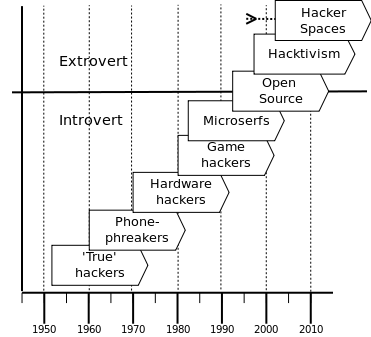
\includegraphics[height=65mm]{hacker-generations-divided.png}

Générations de hacker. Source: Taylor\footnote{Taylor,  P.A. (2005). From hackers to hacktivists: speed bumps on the global  superhighway? New Media \& Society, 7(5):625} Modifié\footnote{http://extreme.ajatukseni.net/tag/hackerspace/}.
\end{center}

Ce projet a, entre autre, le soutien du Président du Conseil d'Administration de l'ULB, du Doyen de la Faculté des Sciences, du Département Informatique, du Cercle Informatique, du Bureau des Étudiants en Sciences, du Bureau des Étudiants Administrateurs ainsi que de plus de 200 étudiants à l'ULB. Globalement, nous proposons de créer une structure non directive favorisant la créativité des étudiants en fournissant la logistique nécessaire pour que les projets aboutissent.

\section{Exemples concrets}

Voici quelques réalisations d'autres hackerspaces qui intéressent déjà nos membres :
\begin{description}
\item[RepRap]\footnote{http://en.wikipedia.org/wiki/Reprap} Une imprimante 3D professionnelle coûte plusieurs milliers d'euro, elle permet notamment de faire du 'rapid prototyping' : c'est un outil de choix dans un atelier. Un projet DIY existe depuis plusieurs années visant à faire les plans d'un tel outil pouvant se répliquer lui-même, d'où le nom. Actuellement, elle est façonnable pour environ 500 euro.

\begin{center}
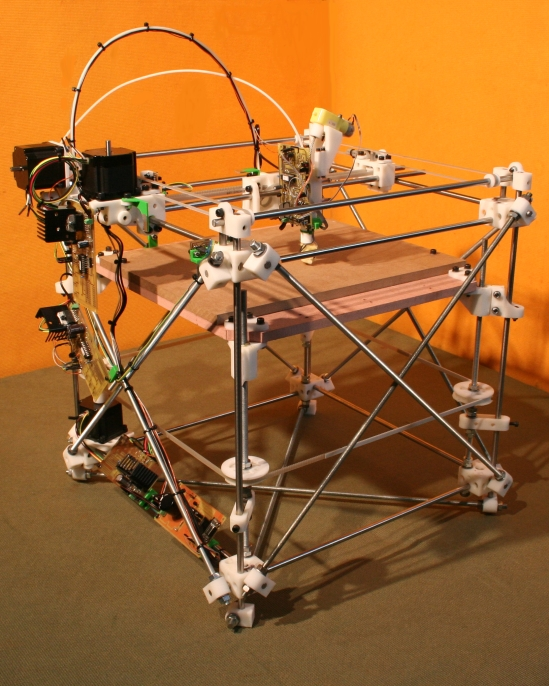
\includegraphics[height=70mm]{reprap-darwin.jpg}

Une reprap. Source: Wikipedia\footnote{http://upload.wikimedia.org/wikipedia/commons/thumb/f/f8/Reprap\_Darwin.jpg/220px-Reprap\_Darwin.jpg}
\end{center}

\item[LaserCuter]\footnote{http://floridacreatives.com/barcamp/laser-cutter-familab-hackerspace} Et toutes les variantes des CNC homemade sont d'autres cibles évidentes pour un laboratoire de ce type.
\item[VendingMachine] Pour organiser la vente des composants électroniques nécessaire à la réalisation de projet sans nécessairement avoir une caisse et un responsable à tout moment, le NYResistor\footnote{http://www.nycresistor.com/2010/01/22/parts-vending-machine/} (hackerspace de New York) a détourné un distributeur de friandises. Cette vending machine est un parfait exemple de réutilisation d'appareil usagé.
\item[LockRFID] La technologie RFID prend une place de plus en plus grande dans nos vies et soulève des questions éthiques relatives à la protection de la vie privée évidentes. L'étude de ces questions pourrait être abordée par exemple en réalisant un système de serrure et de carte RFID ouvrant certaines armoires du hackerspace.
\item[iRail]\footnote{http://www.irail.be/route/} Projet du Whitespace, hackerspace gantois, visant à rendre utilisable les sites publics (surtout celui de la SNCB). Un projet ayant la même philosophie a été réalisé par un étudiant portant le projet hackerspace dans le but de rendre utilisable GeHoL.
\item[Visiter le CERN] L'avantage de la structure non directive est qu'il est possible d'organiser des projets immatériels, par exemple plusieurs étudiants du projet planifient une visite au CERN.
\end{description}

Une partie importante des projets initiaux du hackerspace sera avant tout de fabriquer des outils et de réparer de l'équipement de seconde main pour compléter le workshop.

\section{Avantages pour l'ULB}

Le hackerspace peut notamment apporter à l'ULB : 
\begin{itemize}
\item Implication plus importante des étudiants dans la vie active de l'ULB.
Actuellement, en dehors du foklore et des cercles politiques peu d'initiatives existent afin d'impliquer les étudiants\footnote{L'ULB
propose toute une série d'activités culturelles, mais comme un sondage réalisé par le CI parmi les étudiants BA1, BA2
le montre, ça fait partie des activités extra-scolaires les moins populaires},
avec un laboratoire ouvert aux étudiants, nous pensons que cela diminuera le décrochage
scolaire en suscitant la curiosité et l'envie d'apprendre.
\item Augmentation de la visibilité et du rayonnement de l'ULB dans certains domaines technologiques,
Par exemple, plusieurs universités de part le monde sont connues
principalement grâce au hackerspace qu'elles hébergent, dans la communauté informatique.
\item Ce projet présentant des aspects intéressants pour les polytechniciens, les informaticiens,
les architectes ou encore les physiciens, sa mise en place permettra de créer un nouvel endroit d'émulation
et d'échanges interfacultaires.
\item Ce projet visant à la construction d'équipement pointu, il pourrait être utilisé dans le cadre d'autres projets étudiants par les facultés (par exemple, un travail sur les moteurs pas à pas sur une imprimante 3D)
\end{itemize}

\section{Infrastructure}

Pour fonctionner, le hackerspace a besoin d'un local, d'électricité 
(sur plusieurs circuits si possible), d'eau et d'internet. Une indépendance concernant les heures d'ouvertures serait utile.

Par ailleurs, le local sera divisé en deux parties, l'une à but social favorisant la communication, les débats et échanges d'idées, l'autre à but pratique, plus studieuse permettant la réalisation des idées engendrées lors des discussions. 

Dans la salle sociale, il y aura un frigo, une machine à café, un tableau blanc, 
des armoires pour stocker le matériel important. Dans les deux parties, il faudra des tables et des chaises ainsi que des étagères.

\section{Gestion de l'argent}
\subsection{Financement}

Plusieurs systèmes de financement sont prévus :
\begin{description}
\item[Financement initial]
Au quotidien, peu de fonds de roulement sont nécessaires, à contrario l'investissement de départ sera conséquent afin de lancer le projet.
\item[Cotisation de membres] annuelle, avec un prix faible, donnant le status de membre. 
Ce statut permet de participer au processus décisionnel et d'ouvrir le hackerspace.
L'objectif de la cotisation est aussi de responsabiliser les membres.
\item[Dons d'argent] de particuliers ou d'associations voulant soutenir notre action.
\item[Levée de fonds] pour un projet spécifique (achat de matériel...) C'est 
le même principe que le précédent, sauf que les généreux donnateurs auront la 
garantie que leur argent sera employé dans un but précis.\end{description}

\subsection{Ventes}

Sur place, il sera possible d'acheter des boissons (café, club mate, coca... - 
pas de boisson alcolisée) ainsi que des collations (snickers, mars, lion, chips..).
Il sera aussi possible d'acheter des composants électroniques pour les besoins des projets.


\section{Structure}

Le hackerspace est composé d'un mainteneur, d'un conseil d'administration et des membres.
Le mainteneur est délégué au Cercle Informatique de l'ULB, le hackerspace est 
une sous- structure du-dit cercle, principalement pour des raisons d'assurance,
de responsabilité et pour avoir le status d'ASBL. Par contre, les deux groupes de 
membres (membre du cercle, membre du hackerspace) seront séparés, étant donné que 
les deux populations sont différentes (et indifférentes à l'existence de l'autre). 
L'élection du mainteneur et du conseil d'administration sera réalisée par les 
membres du hackerspace.

\section{Objectifs et méthodes}

Le hackerspace souscrit au principe du libre examen et aux autres valeurs de l'ULB.
Il souscrit aussi à une idée de liberté dans un sens plus large en encourageant et en promulguant l'usage de logiciels libres, la neutralité d'Internet, le partage et l'ouverture de 
l'information et plus généralement l'accès universel, libre et gratuit aux connaissances.

Le hackerspace est conscient qu'il présente peu d'intérêt si isolé. Il cherche donc 
à s'inscrire dans une logique de continuité et à s'intégrer aux réseaux d'hackerspaces 
internationaux.

Le hackerspace, pour évoluer, doit notamment connaitre sa propre histoire : il est 
donc très important de disposer d'archives ouvertes et entretenues de manière 
automatique (cf. incubator). Plus spécifiquement, des statistiques seront 
conservées pour mettre en évidence les contributions des membres et leurs conséquences. 
Il doit aussi être à l'écoute de tous ses membres et fournira des moyens simples pour 
donner un feedback. 

Pour vivre et s'enrichir harmonieusement, le hackerspace doit disposer d'une base 
règlementaire. Il est évident que le hackerspace respectera les règles de l'ULB 
(charte horaire, réglementation au niveau de la sécurité ou du tabac). De plus, il souscrit aux 
design patterns\footnote{http://hackerspaces.org/wiki/Design\_Patterns}
\footnote{https://hackerspace.be/Patterns} reconnus et plus généralement à une 
éthique\footnote{http://en.wikipedia.org/wiki/Hacker\_ethic}, sauf si c'est en 
contradiction avec sa situation spécifique.


\section{Thèmes}

Sujets proposés comme base de travail, pistes purement indicatives, lors des 
conférences et des workshops (liste non exhaustive) :
\begin{itemize}
\item Programmation avancée
\item Administration système et réseau
\item Lifestyle, lifehacking
\item Hardware hacking
\item Electronique et interfaçage avec un ordinateur (arduino..)
\item Radio-identification (technologie RFID)
\end{itemize}

\section{Processus}
\subsection{Incubator}

Il existe trois types de personnes potentiellement interessées par le hackerspace :
\begin{itemize}
\item Une personne ayant envie de travailler en groupe sur un projet, mais qui ne 
sait pas trop quoi (personne motivée mais sans idée)
\item Une personne qui a une idée précise mais manque de moyen technique, 
le hackerspace répond à ses besoins
\item Une personne qui a une idée précise mais manque de moyen humain : 
la première catégorie de personne répond à ses besoins
\end{itemize}

Dans le but de faciliter la mise en commun et d'augmenter la chance qu'un projet 
arrive à terme, il faudra mettre en place un incubator, un service en ligne permettant :
\begin{itemize}
\item de lister l'ensemble des membres motivés avec leurs compétences et leurs 
centres d'intérêts, pour avoir une vision d'ensemble
\item de visualiser les projets (définition, explications, roadmap, info utiles...) 
du hackerspace en cours et en planification
\item de permettre à tous d'adhérer à un ensemble de projets auquel il est prêt à s'investir.
\item de lancer les projets qui ont atteint un seuil critique de définition et 
de gens prêts à travailler dessus
\item de coordonner la workforce sur plusieurs projets en cas de mise en pause forcée d'un autre
\end{itemize}

Cette méthode de travail, en plus d'augmenter la productivité générale, permettra 
à des gens de rapidement s'intégrer facilement à la structure en place en diminuant 
le temps de "découverte" du hackerspace.

\subsection{Quibossocratie}

Méthode employée par des groupes au moyen humain très limité : si quelqu'un prend 
une initiative, travaille, c'est lui qui prend les décisions relatives au projet. 
Cela part de la constatation que l'immobilisme par peur des conséquences est une 
plaie dans toute structure associative et qu'il est plus facile de demander pardon 
que de demander la permission.

Cette méthode n'implique pas forcément une abscence de dialogue ni d'entente. 
C'est juste pour limiter les "il faut que", "Il n'y a qu'à", "on ne devrait pas lancer...": Just do it.

\subsection{Gestion des gens, heures d'ouverture, prise de décision}

Il y aura une ou deux soirées par semaine de "grosse" hacking party, dont au moins 
une précédée par une réunion.
Le reste du temps, le hackerspace sera ouvert en après-midi et soirée selon les 
besoins et les disponibilités.
Une fois par mois, le hackerspace organisera une conférence.

\newpage
\section{Historique}

Au premier semestre nous étions plusieurs étudiants voulant monter un hackerspace.
Pour ce faire nous nous sommes lancés dans l'organisation de linux install party et
de coding party dans le but de réunir des gens motivés pour lancer le projet autour
autour de ce noyau.

Puis, suite à une rencontre avec Markus Lindström et Stephane Fermandes Medeiros, assistants au DI, ces derniers nous ont convaincus de la faisabilité d'avoir un local à
l'ULB si nous présentions un projet concret et sérieux. Nous changeons alors de mode
opératoire pour en faire un projet infrastructure-driven (endroit, connectivité, serveurs..),
l'histoire montrant que cela rend ce type de projet plus viable.  Au départ, les deux
assistants  sus-nommés voulaient fonder un laboratoire pédagogique interfacultaire,
dont le hackerspace serait une composante. Maheureusement depuis, ce projet plus
global a été mis en attente.

Fin février, nous avons lancé un site web\footnote{http://hackerspace.cerkinfo.be} comportant
une invitation à signer une pétition de soutien pour notre projet. La nouvelle s'est répandue rapidement parmi les intéressés; actuellement, cette pétition recueille le soutien de plus de 220 étudiants ainsi que celui d'une dizaine de membres du corps académique.

Depuis, ce projet a obtenu le soutien du président du CA, de la Doyenne de la Faculté des Sciences, du département informatique,du 
cercle informatique ainsi que du bureau des étudiants en sciences et du bureau des étudiants administrateurs.
De plus, plusieurs membres du BEP ainsi que de certains services de la facultés
des sciences appliquées (CoDE, OPERA notament) ont également apporté leur soutien personnel.

\section{Conclusion}
Nous pensons que l'ouverture d'un hackerspace à l'ULB serait une véritable opportunité pour notre alma mater. En effet, sa création comblerait un véritable manque de structure par les étudiants pour les étudiants désirant s'investir et mettre en pratique les connaissances acquises lors de leur cursus. Véritable lieu de partage, d'échange et d'émulation pour les passionnés, en plus de tous les avantages qu'une structure du genre apporterait aux étudiants, il pourrait être un rayonnement supplémentaire pour l'université dans les milieux spécialisés.

Nous avons la conviction qu'avec ce projet, notre Université ne pourrait qu'en ressortir grandie.


\end{document}
